% Historique du sujet
% Introduction théorique
% Application dans la vie courante
Le mouvement de rotation est l'un des deux mouvements fondamentaux dans l'étude des mouvements en physique (le second étant le mouvement rectiligne). Le moment d'inertie est une mesure de la résistance d'un objet au mouvement de rotation. En effet, la cinématique de rotation s'applique lorsque toutes parties d'un corps tournent autour d'un axe, mais nous ne nous concentrerons que sur celle effectuant une rotation angulaire constante ou uniformément accéléré autour d'un axe fixe. Un objet en rotation possède une inertie déterminé par la forme de celui-ci. \\ \\
Ce phénomène peut se retrouver dans la physique d'un yoyo, d'une toupie à fil. Sans inertie, le yoyo tomberait à le même vitesse que s'il était lâché (sans le support du fil); tirer le fil de la toupie ne demanderait quasiment aucune énergie. Dans un cadre plus commun, la notion d'inertie est utile dans la conceptions de pneus, car cela déterminera la difficulté pour le mettre en mouvement ou alors l'arrêter.\\ \\
% D'un point de vue plus pratique, lorsque l'on démarre une tondeuse, nous tirons sur un une corde afin de faire tourner un disque. Une résistance du disque sera ressentie due à l'inertie, et cette énergie provenant de la résistance permettra de commencer la combustion et du mise en mouvement du moteur.\\
Avant Galilée, le théorie du mouvement ne connaissait pas l'inertie: l'état d'un corps est immobile dans son ``lieu naturel'' et son ``mouvement naturel'' est de retourner dans son milieu. Ainsi, les corps lourds tel que l'eau et la terre devait tomber, et les corps légers comme l'air ou le feu devait monter. Les anciennes idées de conservation du mouvement d'Aristote seront reprises, celles-ci expliquait qu'en projetant un projectile, ce dernier peut conserver en lui de l'élan. Newton s'inspire des écrits de Galilée et Descartes afin de proposer sa vision de l'inertie, qui est sa première loi : tout corps persévère dans l'état de repos ou de mouvement uniforme en ligne droite dans lequel il se trouve, à moins que quelque force n'agisse sur lui, et ne le contraigne à changer d'état. Huygens va définir le moment d'inertie qui s'applique similairement aux objets en rotations\footnote{\href{https://fr.wikipedia.org/wiki/Inertie}{Source : \textit{https://fr.wikipedia.org/wiki/Inertie}}}.\\ \\
L'inertie découle de la deuxième loi de Newton:
$$
    \sum{\vec{F}} = m \vec{a}
$$
Dans le cas où un objet tourne autour d'un axe, une formule similaire est utilisée:
$$
    M = I \alpha 
$$
avec $M$ [$N \cdot m$] le moment de force, $\alpha$ [$rad(1/s^2$)] l'accélération angulaire et $I$ [$kg \cdot m^2$] le moment d'inertie. (Notons que cette formule est un cas particulier que le solide tourne autour d'un axe, mais une expression générale existe également avec un tenseur d'inertie.)\\ \\
Chaque objet possède une inertie différente dépendant de sa masse, sa taille et le placement de l'axe auquel il tourne autour. Lors de l'expérience, nous utilisons un ``disque'' (en soit un empilement de disques) placé sur un coussin d'air, équivalant à un axe de rotation vertical.

\begin{figure}[H]
  \centering
  \begin{minipage}[b]{0.4\textwidth}
    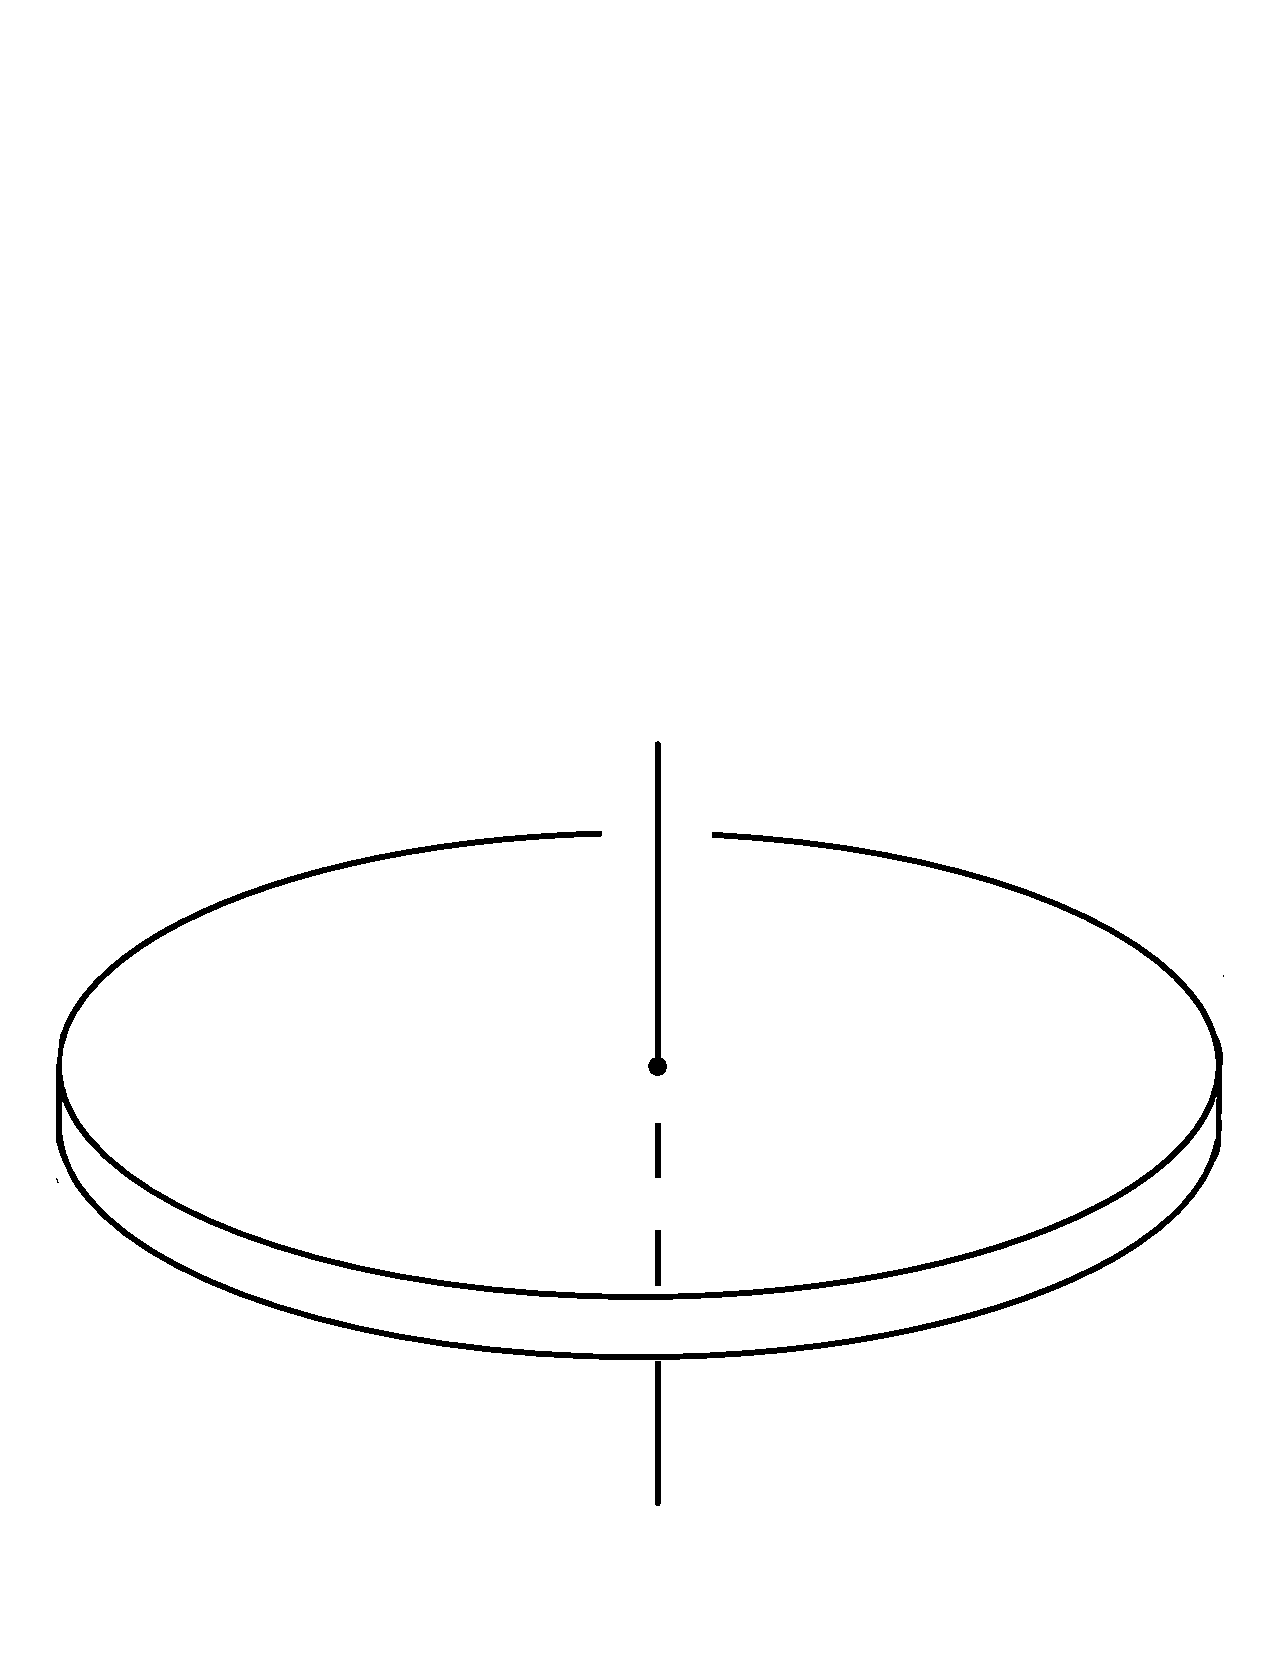
\includegraphics[width=\textwidth]{Phy_rot_disque1.pdf}
    \caption{Un disque ayant un axe de rotation vertical a une inertie valant $I = \frac{r^2}{2}$}
  \end{minipage}
  \hfill
  \begin{minipage}[b]{0.4\textwidth}
    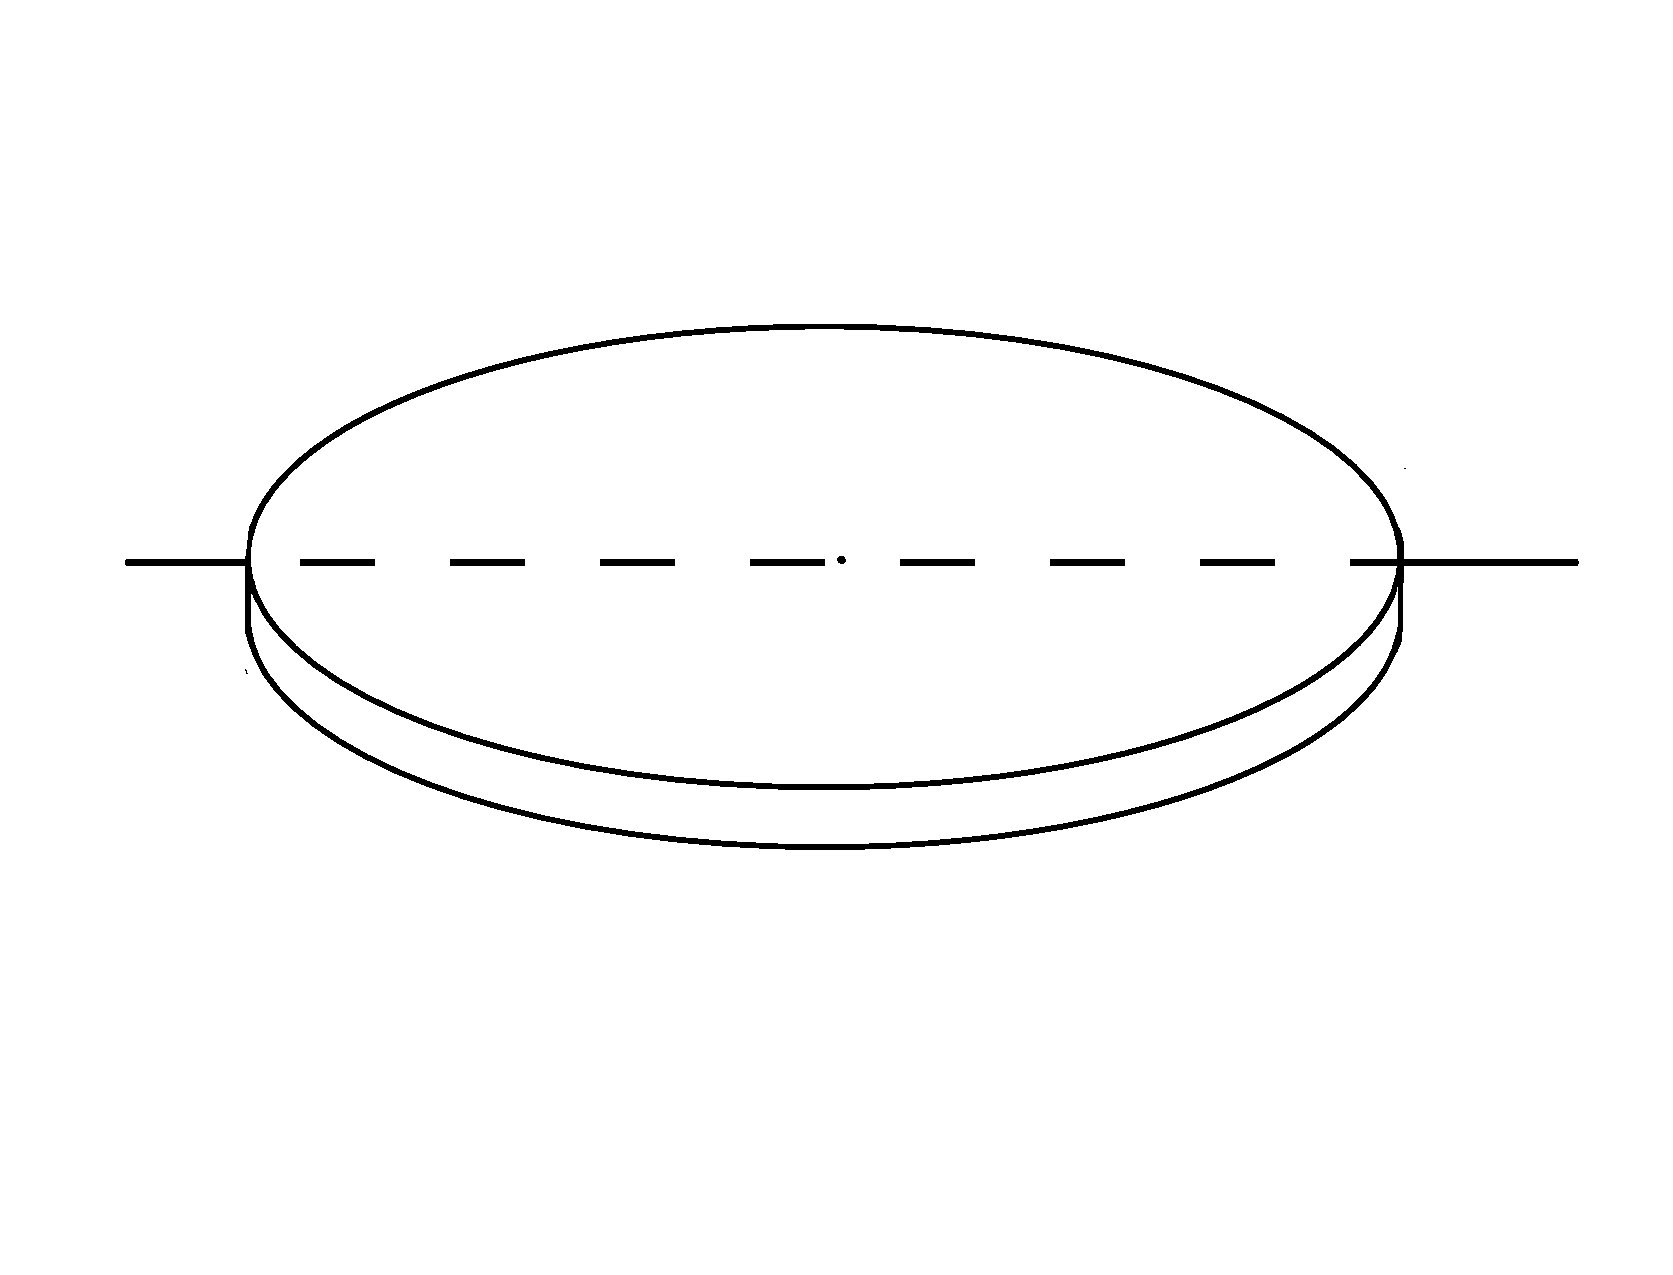
\includegraphics[width=\textwidth]{Phy_rot_disque2.pdf}
    \caption{Un disque ayant un axe de rotation horizontal a une inertie valant $I = \frac{r^2}{4}$}
  \end{minipage}
\end{figure}

Un point placé sur un disque en rotation peut être caractérisé par une trajectoire circulaire accéléré, ou non. Dans un mouvement circulaire uniforme (\textit{MCU}), un point matériel à une position $\theta_0$ [$rad$] de sa référence, subie une vitesse angulaire constante $\omega_0$ [$\frac{rad}{s}]$ autour d'un axe:
$$
    \theta(t) = \omega_0 t + \theta_0
$$
et dans le cas d'un mouvement uniformément accéléré (\textit{MCUA}), nous prenons compte d'un $\alpha$, représentant la constante d'accélération angulaire du système:
$$
    \theta(t) = \frac{1}{2} \alpha t^2 + \omega_0 t + \theta_0
$$
